\documentclass[a4paper,12pt]{book}
\usepackage[utf8]{inputenc}
\usepackage[margin=24mm]{geometry}

\usepackage{float}
\usepackage{graphicx}
\graphicspath{ {images/} }

\usepackage[
backend=bibtex,
style=alphabetic,
citestyle=authoryear,
autocite=inline
]{biblatex}

\addbibresource{references/references.bib}

\usepackage{helvet}
\usepackage{subfig}

\usepackage[Lenny]{fncychap}
\usepackage{xcolor}


\begin{document}

\frontmatter
%----------------------------------------------------------------------------------------
%	TITLE PAGE
%----------------------------------------------------------------------------------------

\newcommand*{\titlePage}{\begingroup % Create the command for including the title page in the document
	\fontfamily{phv}\selectfont
	\centering % Center all text
	
	\vspace{200pt}
	{\Huge Developing an educational tool to promote evidence-based treatment in health care} \\ % Title
	\vspace{5pt}
	
	{\Large \textsl{A pilot study}} % Subtitle or further description
	\vspace{50pt}
	
	{\Large{Ben-Richard Sletten Ebbesvik}}\\ % Author name
	
	\vfill % Whitespace between the author name and the publisher logo
	
	{\Large Research proposal for master's thesis in Software Engineering at \\
		\vspace{10pt}
		Department of Computing, Mathematics and Physics, \\
		Bergen University College \\
		\vspace{10pt}
		Department of  Informatics, \\
		University of Bergen \\}
	\vspace{10pt}
	{\large April 2018} % Month and year published
	
	\begin{figure}[h!]
		\captionsetup[subfigure]{labelformat=empty}
		\subfloat[][]{
\includegraphics[width=250pt]{images/hvl_logo_engelsk.pdf}}
		\hfill
		\subfloat[][]{
\includegraphics[width=70pt]{images/uib-logo.pdf}}
	\end{figure}
	
	
	\endgroup}
\titlePage

\tableofcontents
\mainmatter


\section{Paper publication}
In December 2018, we submitted a paper "A Model Driven Approach to the Development of Gamified Interactive Clinical Practice Guidelines", which was a summary of our work so far in this project and related projects. The paper was accepted for publication by ENASE 2019 – 14th International Conference on Evaluation of Novel Approaches to Software Engineering, where we held a presentation on their conference in Heraklion, Greece. 

The paper can be found in appendix \ref{appendix:Paper} in this thesis.

%\section{Old Research questions}
%\begin{itemize}
	%\item Can we make a data structure representing the paediatric possible asthma guideline \parencite{RepublicofKeny2016}  in a very generic way?
	%\item Based on the data structure, can we generate suitable scenarios, with multiple choice %question with answer elements for training and evaluating health personnel?
	%\item How can we structure the learning material to best train medical students, doctors, clinical officers, nurses and other health workers in the paediatric possible asthma guideline \parencite{RepublicofKeny2016}? 
			%\item Based on clinical guidelines, can we make a reusable data structure representing respiratory diseases for use in serious games?


%-------
%	\item Based on clinical guidelines, can we make a data structure which is easy to implement in the system, as well as adaptable? 
	
%	\item How to use such a model for generating and testing case based multiple choice questions and answer elements?
	%\item Can we use the data model to structure the learning content such that it is adapted to the current knowledge of the individual learner?
	
	
%	\item How can we model the work-flow of a clinical encounter, a patient at a given point in the clinical encounter, and a student at the current point in his learning process. How to represent these?	
%\end{itemize}

%\textcolor{purple}{TODO Yngve: Gamification, hva evaluerer du?}


\section{Research questions}

\begin{itemize}
	\item \textbf{RQ1:} Based on clinical guidelines, how can we define and represent a generic data structure that can be used to implement applications such as online guidelines or training games for such guidelines, and where applications can adapt to the level of their users?
	\item \textbf{RQ2:} Can the generic data structure in RQ1 be used to generate a specific data model for another domain such as paediatric asthma?
	\item \textbf{RQ3:} How can we use the data model in RQ2 to implement a game for guideline training that can adapt to the level and progression  of users?
	\item \textbf{RQ4:} Is the guideline meta model at an abstraction level such that it can be used for other guidelines? 
\end{itemize}
\section{Structure of the thesis}
\section{Summary}
Here we have defined a set of research questions, which is related to the development of serious games for clinical guidelines. Making games which are adaptable to the knowledge level, progression of the user, and making guideline models which are at an abstraction level where they can be used to represent other CPGs, are the main focus points.

We have also given a short presentation of each chapter in the thesis.



\section{Clinical Practice Guidelines}
\textcite{Fervers2010} claims that for clinicians, increased medical knowledge is associated with an exponential growth of scientific data and published material. It is impossible to keep up, as well as integrating all the new information into daily practice to give patients the best possible care.  \textcite{Masic2008} gives an example where a general practitioner should read 19 articles per day to keep up with the new medical information, while only having time for reading one hour per week. Reading 19 articles per day, would acquire more time than the clinician has available for treating patients. This problem is known as academic isolation \parencite{Masic2008}.

Evidence Based Medicine (EBM) suggests that instead of routinely reading dozens of articles, the clinicians should target their reading to specific patient problems. Developing clinical questions and then searching for the answer (problem based approach) may be a more productive way to keep up with the new medical knowledge \parencite{Masic2008}. The EBM definition further puts an emphasize on integrating the best evidence in decision making with the clinicians expertise and the patients values and expectations \parencite{Masic2008}. 

The concept of EBM is about transferring knowledge from clinical research into clinical practice, and Clinical Practice Guidelines (CPG) can play an instrumental role in this process \parencite{Fervers2010}.

The Institute of Medicine (IOM) has given the following definition of clinical practice guidelines: "CPGs are statements that include recommendations intended to optimize patient care. These statements are informed by a systematic review of evidence and an assessment of the benefits and costs of alternative care options" \parencite{Guidelines2011}

The definition given by IOM covers the goals in EBM, and also takes the cost into account. In fact, \textcite{Clayton1995} have shown that in some situations good use of appropriate guidelines and protocols can reduce as much as 25\% of the cost of healthcare.

% I can use Woolfs article and write even more about benefits. Should probably do that.

Even though the CPGs have proven to improve the quality of health care while reducing practice variability and the cost of patient care \parencite{DeClercq2008}, it is well recognized that CPGs have had a limited effect on changing the clinicians practice methods. \textcite{Cabana1999} lists the following reasons:
\begin{itemize}
	\item \textbf{Lack of awareness:} the clinician is not aware of the guideline's existence.
	\item \textbf{Lack of familiarity:} the clinician is not familiar with the content of the guideline.
	\item \textbf{Lack of agreement:} the clinician had various reasons to disagree with the guideline, such as they are oversimplified, disagree with the evidence or not worth the patient risk, discomfort or cost.
	\item \textbf{Lack of self-efficacy:} is the lack of self-confidence in that the clinician can execute the recommendations of the guideline correctly.
	\item \textbf{Lack of outcome expectancy:} the clinician doesn't believe the outcome of the recommended treatment will meet the outcome expectancy.
	\item \textbf{Inertia of previous practice:} the custom, habit or previous training can hinder the adaptation of clinical practice.
	\item \textbf{External Barriers:} the guidelines are not easy to use, not convenient, cumbersome and confusing.
\end{itemize}One example of external barrier is the Guidelines for the Diagnosis and Management of Asthma \parencite{NationalHeartLungandBloodInstitute2007}, which consists of 440 pages. Such a large document is not convenient to use at the point of care. According to \textcite{Shortliffe1998}, CPGs in monographs and journal articles tend to sit on book shelves at the time their knowledge could prove the most valuable to the clinicians. 

\subsection{Discussion}
According to \textcite{Woolf1999}, clinicians sometimes have good reasons to disagree with some of the content of a guideline. \textcite{Woolf1999} points out three reasons:
\begin{enumerate}
	\item The scientific evidence of the recommendation can be lacking, misleading or misinterpreted.
	\item The recommendations may be influenced by the authors. What the authors believe, may be inferior to other options, ineffective or harmful.
	\item As the guideline may be written to control cost, serve societal needs or protect special interest, the recommendations may be suboptimal for the patient.
\end{enumerate}
There exists grading systems which grade the quality of evidence and strength of recommendations. GRADE is such a grading system \parencite{Guyatt2008}. When displaying guidelines to clinicians, it is a strong point to display the grade of evidence, as the clinician has to choose between several treatment options.


%\textcolor{red}{\begin{itemize}
%	\item Medical knowledge increases. Hard to keep track
%	\item Guidelines is a summary of the available evidence of the medical conditions and provide management and recommendations
%	\item A well-developed guideline reduces
%	variations in care, improves diagnostic accuracy,
%	promotes effective therapy and discourages ineffective
%	therapies all which contribute to improved
%	quality of care (citation)
%	\item The CPGs are not used enough
%	\item Dissemination and implementation
%	\item Large volume of excisting guidelines. Difficult to use at the point of care
%	\item Dissemination
%	\item Different practice even in the same country
%\end{itemize}}


\section{Serious games}
When searching the literature for the definition of serious games, there seem to be many different understandings of what serious games really is. However, these definitions seem to have the common understanding that serious games are games which are used for other purposes than just pure entertainment \parencite{Susi2015}. This is actually a very broad category, where we can find games which are used to test job applicants or to improve our health by encouraging us stay more active.

\textcite{Michael2006} defines serious games as "a serious game in which education (in its various forms) is the primary goal, rather than entertainment". \textcite{Michael2006} emphasizes that education and entertainment should not be in conflict, but that they can overlap. The feeling of learning something new or getting better at something, can be quite satisfying and can serve as an entertainment factor.

Serious games also have the advantage over educational books and movies that the student can demonstrate and apply what he has learnt, through tasks in the game \parencite{Michael2006}.    Serious games seem more effective than training with conventional instruction methods, as the knowledge gains persists in the long term memory, and the learner can build on this well-structured prior knowledge through his learning career \parencite{Wouters2013}. However, serious games seems to be most effective when they are supplemented with instructional learning methods. Not only gets the student to learn by doing, but he also gets the opportunity to reflect over what he has learnt and to verbalize the new knowledge, making it easier to integrate it into his knowledge base \parencite{Wouters2013}. 





\section{Motivation}
By making a serious game for clinical practice guideline training, we can address some of the reasons why the CPGs haven't had a greater impact on clinicians practice methods \parencite{Cabana1999}:
\begin{itemize}
	\item \textbf{Lack of awareness:} The more projects around CPGs, the more focus will they get and more people will be aware of their existence. By making a serious game, we may be able to target some user groups which where hard to reach in traditional ways. 
	\item \textbf{Lack of familiarity:} By playing the game, the student will learn more about the content and will become familiar with the CPGs. The student may also be encouraged to study the CPGs in the traditional ways after having played the game.  
	\item \textbf{Lack of self-efficacy:} By repeatedly solving practical tasks in the game, the student may become confident in that they are capable of executing the treatment recommended by the CPG.
	\item \textbf{External barriers:} convenient, cumbersome and confusing CPGs will by approach be converted to a game format. Even though a game isn't a good encyclopaedia at the point of care, for some user groups a game might be a better format for studying. Especially a combination of instructional learning methods and serious games have shown positive learning results \parencite{Wouters2013}. Having built well-structured prior knowledge may also help at the point of care.
\end{itemize}

Another motivational reason for making a serious game is the scalability. How can we best train 10, 100 or 1000 clinicians in the best practices of medical guidelines? There are logistics problems with instructional courses and training sessions, such as cost of money, time and there's a practical limit for how many attendees can attend a course at the same time. A mobile game scales much better as downloading an mobile application is much cheaper, can be played almost anywhere at any time. There's no limitation on how many playing participants.

\subsection{Asthma}
Asthma is a repository disease, which in the recent years have had an almost exponential growth rate among children in Oslo. From 0.4\% in the first Norwegian report, to 8\% in 1993 and 20.2\% in 2006. Similar results were found in the rest of Norway in the early 90s. \parencite{Carlsen2006}. 

Asthma growth amongst children is not only an issue in Norway. According to \textcite{Odhiambo1998}, 3\% of children in rural areas in Kenya had asthma in 1998 and 9.5\% of the children in urban areas. Before this study it was a claim that asthma among African children was rare, which is no longer true \parencite{Odhiambo1998}.

It is urgent to find answers to prevent further increase of asthma amongst children in the years to come\parencite{Carlsen2006}.

As our contribution to put focus on the dramatically growth of asthma in children, our work will centre around the paediatric possible asthma guideline \parencite{RepublicofKeny2016} when developing a serious game to promote guideline training in health care.

\subsection{Challenges}
\section{Related work}
\section{Summary}


\chapter{Method}
\section{Design study}

\section{Focus group}
\section{Workshop}
The 22nd of February we had a workshop. The purpose of the workshop was to
\begin{itemize}
	\item Identify components in the treatment plan of asthma patients.
	\item Identify difficulty levels, and how the questions will be more detailed for every difficulty level.
	\item Make a learning map.
\end{itemize}

The antecedences for the meeting was 
\begin{itemize}
	\item Professor in computer science Yngve Lamo. Background in model driven engineering and health informatics.
	\item Assistant professor in computer science Svein Ivar Lillehaug. Background in health informatics.
	\item Postdoctoral fellow Fazle Rabbi. Background in model driven engineering.
	\item Medical doctor and PhD student in health informatics Job Nyangena.
	\item PhD research fellow in interaction design Rosaline Barendregt. Has written a master thesis in gamification.
	\item PhD candidate in computer science Suresh Kumar Mukhiya.
	\item Master degree student in computer science Ben-Richard Ebbesvik.	
\end{itemize}



\begin{figure}[h]
	\caption {Anticlockwise from front left: Yngve Lamo, Rosaline Barendregt, Suresh Kumar Mukhiya, Svein Ivar Lillehaug, Fazle Rabbi and Job Nyangena}
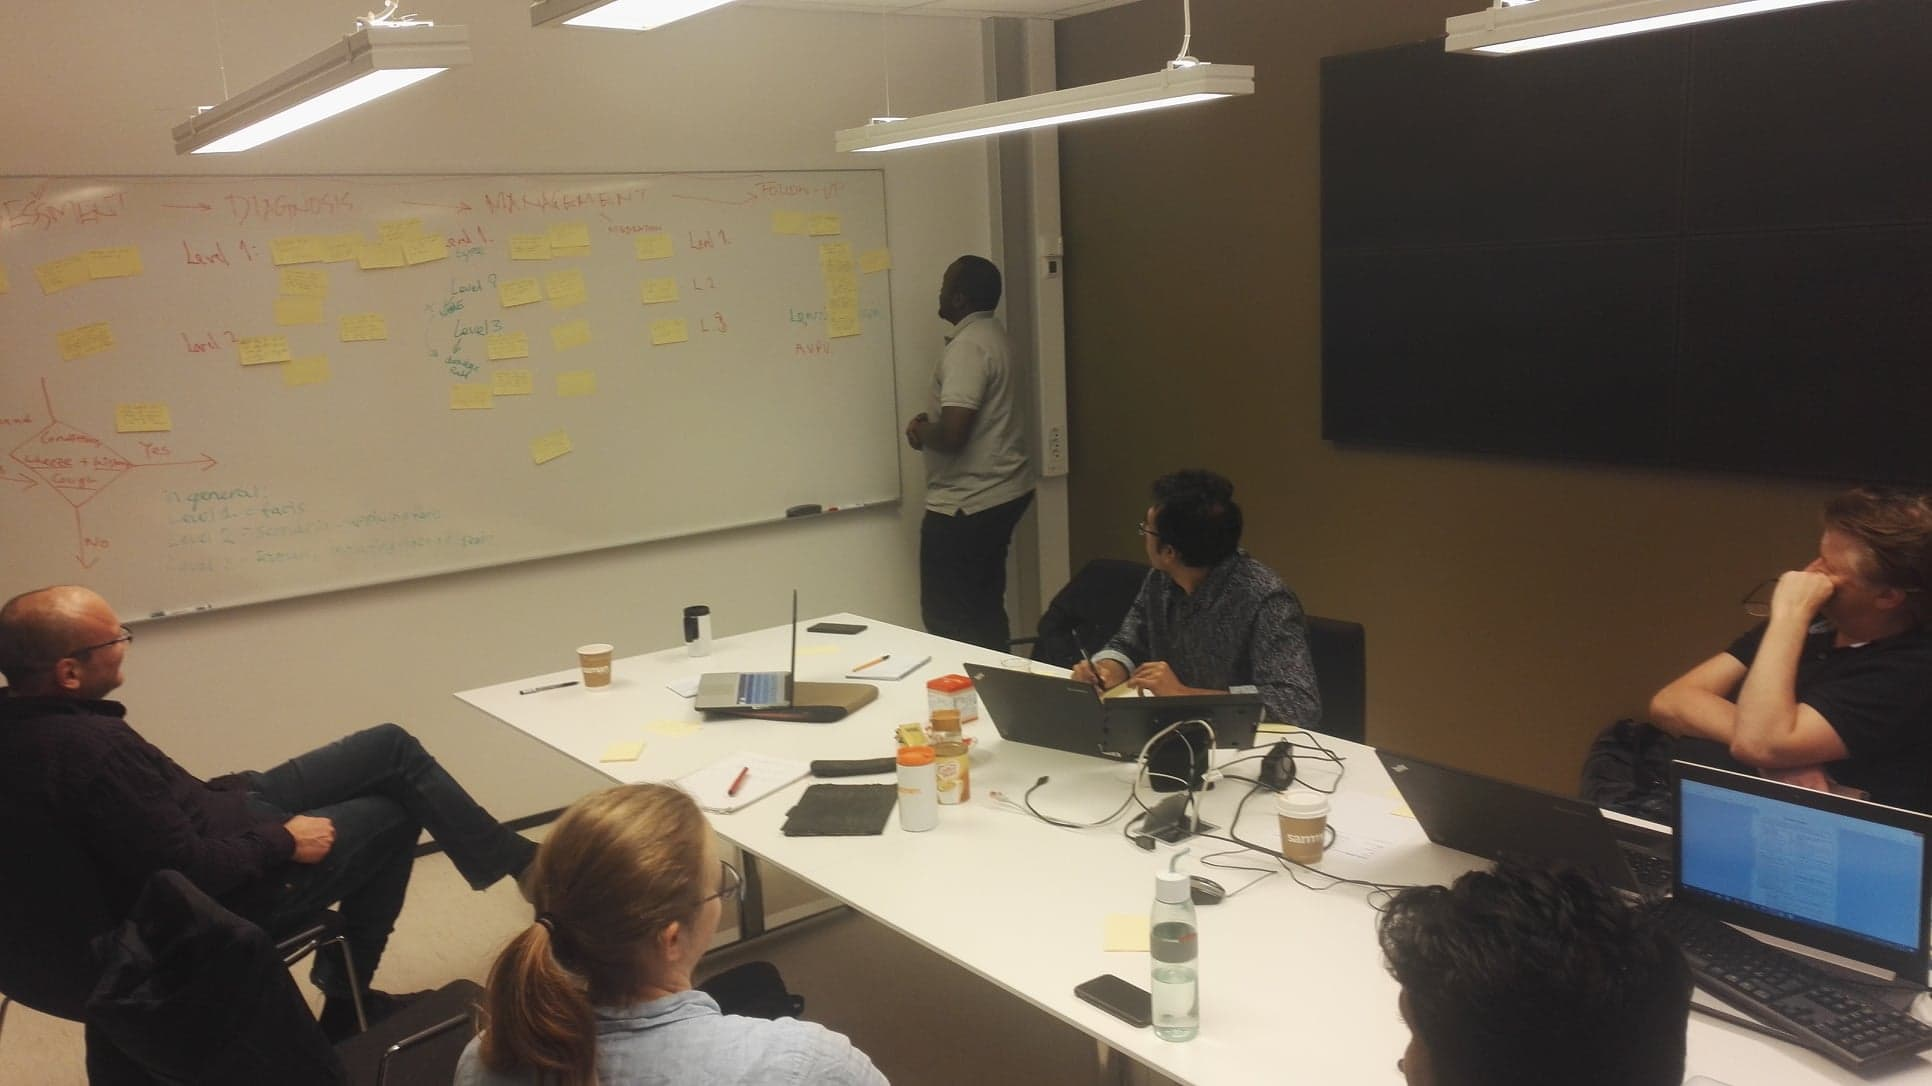
\includegraphics[scale=0.25]{workshop220219}
\end{figure}

\begin{figure}[h]
	\caption {Workshop with Yngve Lamo, Rosaline Barendregt, Suresh Kumar Mukhiya, Svein Ivar Lillehaug, Fazle Rabbi and Job Nyangena}
	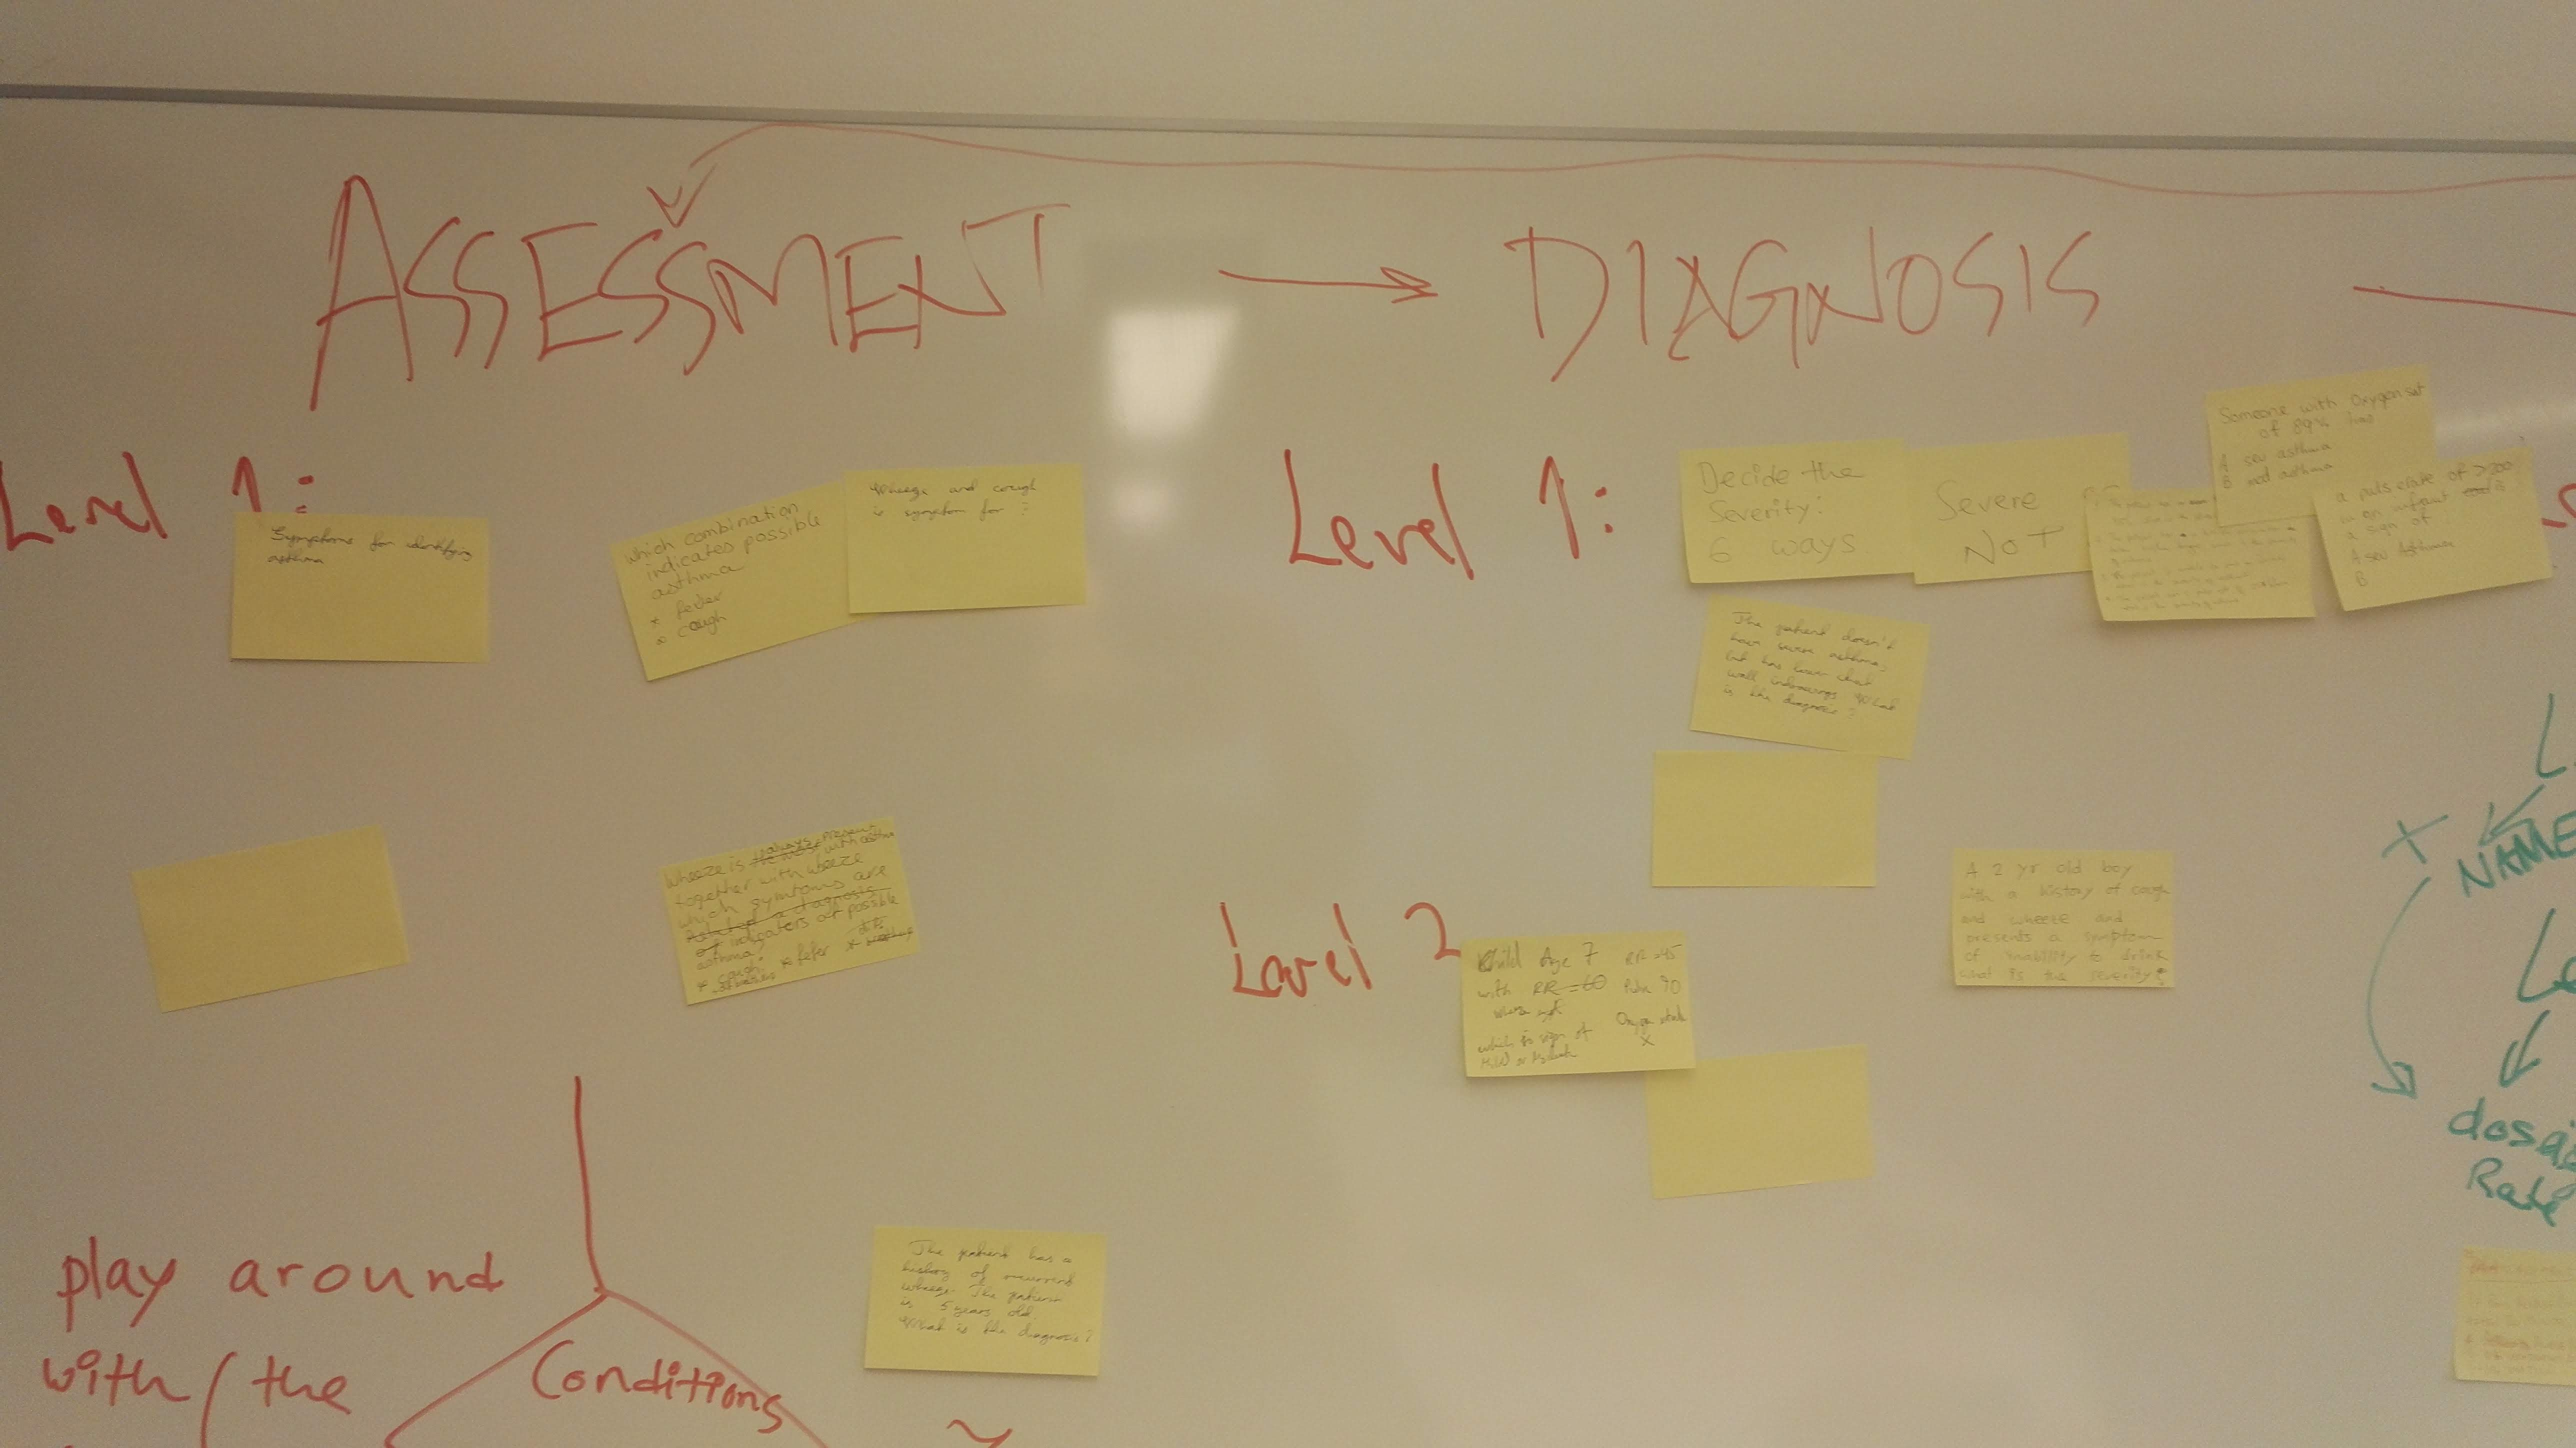
\includegraphics[scale=0.075]{workshop220219-2}
\end{figure}

\begin{figure}[h]
	\caption {Workshop with Yngve Lamo, Rosaline Barendregt, Suresh Kumar Mukhiya, Svein Ivar Lillehaug, Fazle Rabbi and Job Nyangena}
	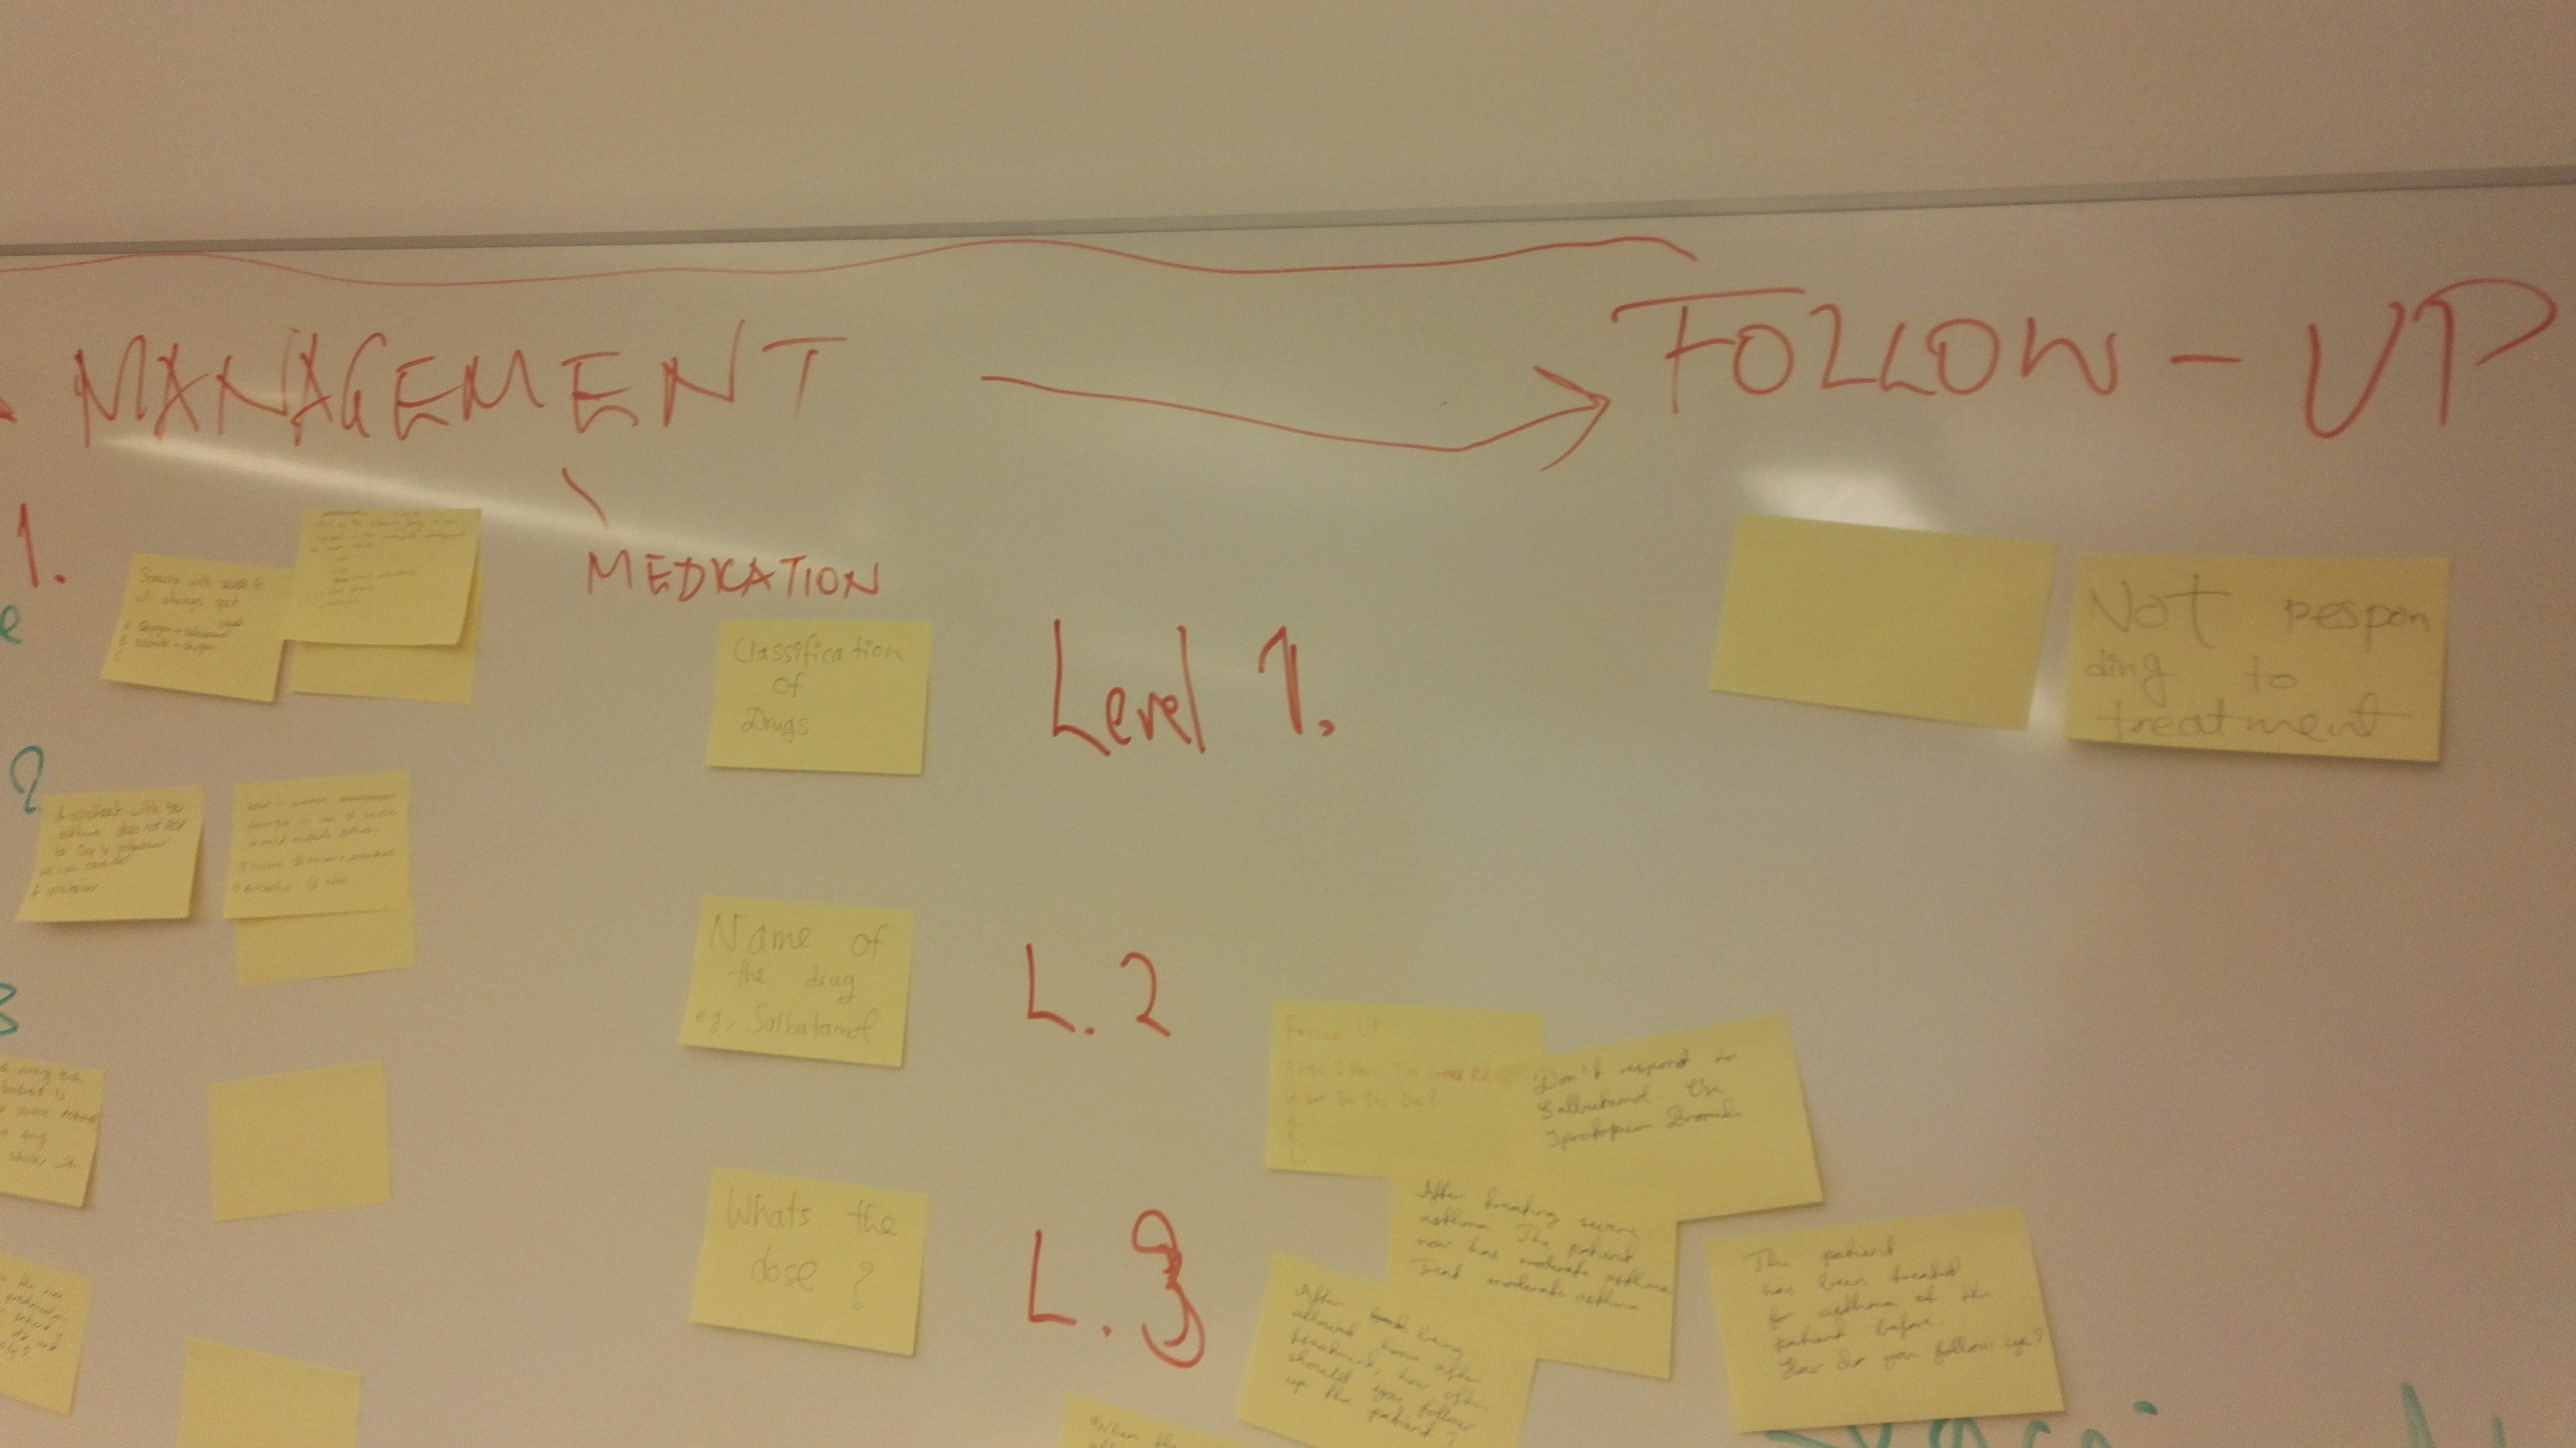
\includegraphics[scale=0.075]{workshop220219-3}
\end{figure}

\begin{figure}[h]
	\caption {Workshop with Yngve Lamo, Rosaline Barendregt, Suresh Kumar Mukhiya, Svein Ivar Lillehaug, Fazle Rabbi and Job Nyangena}
	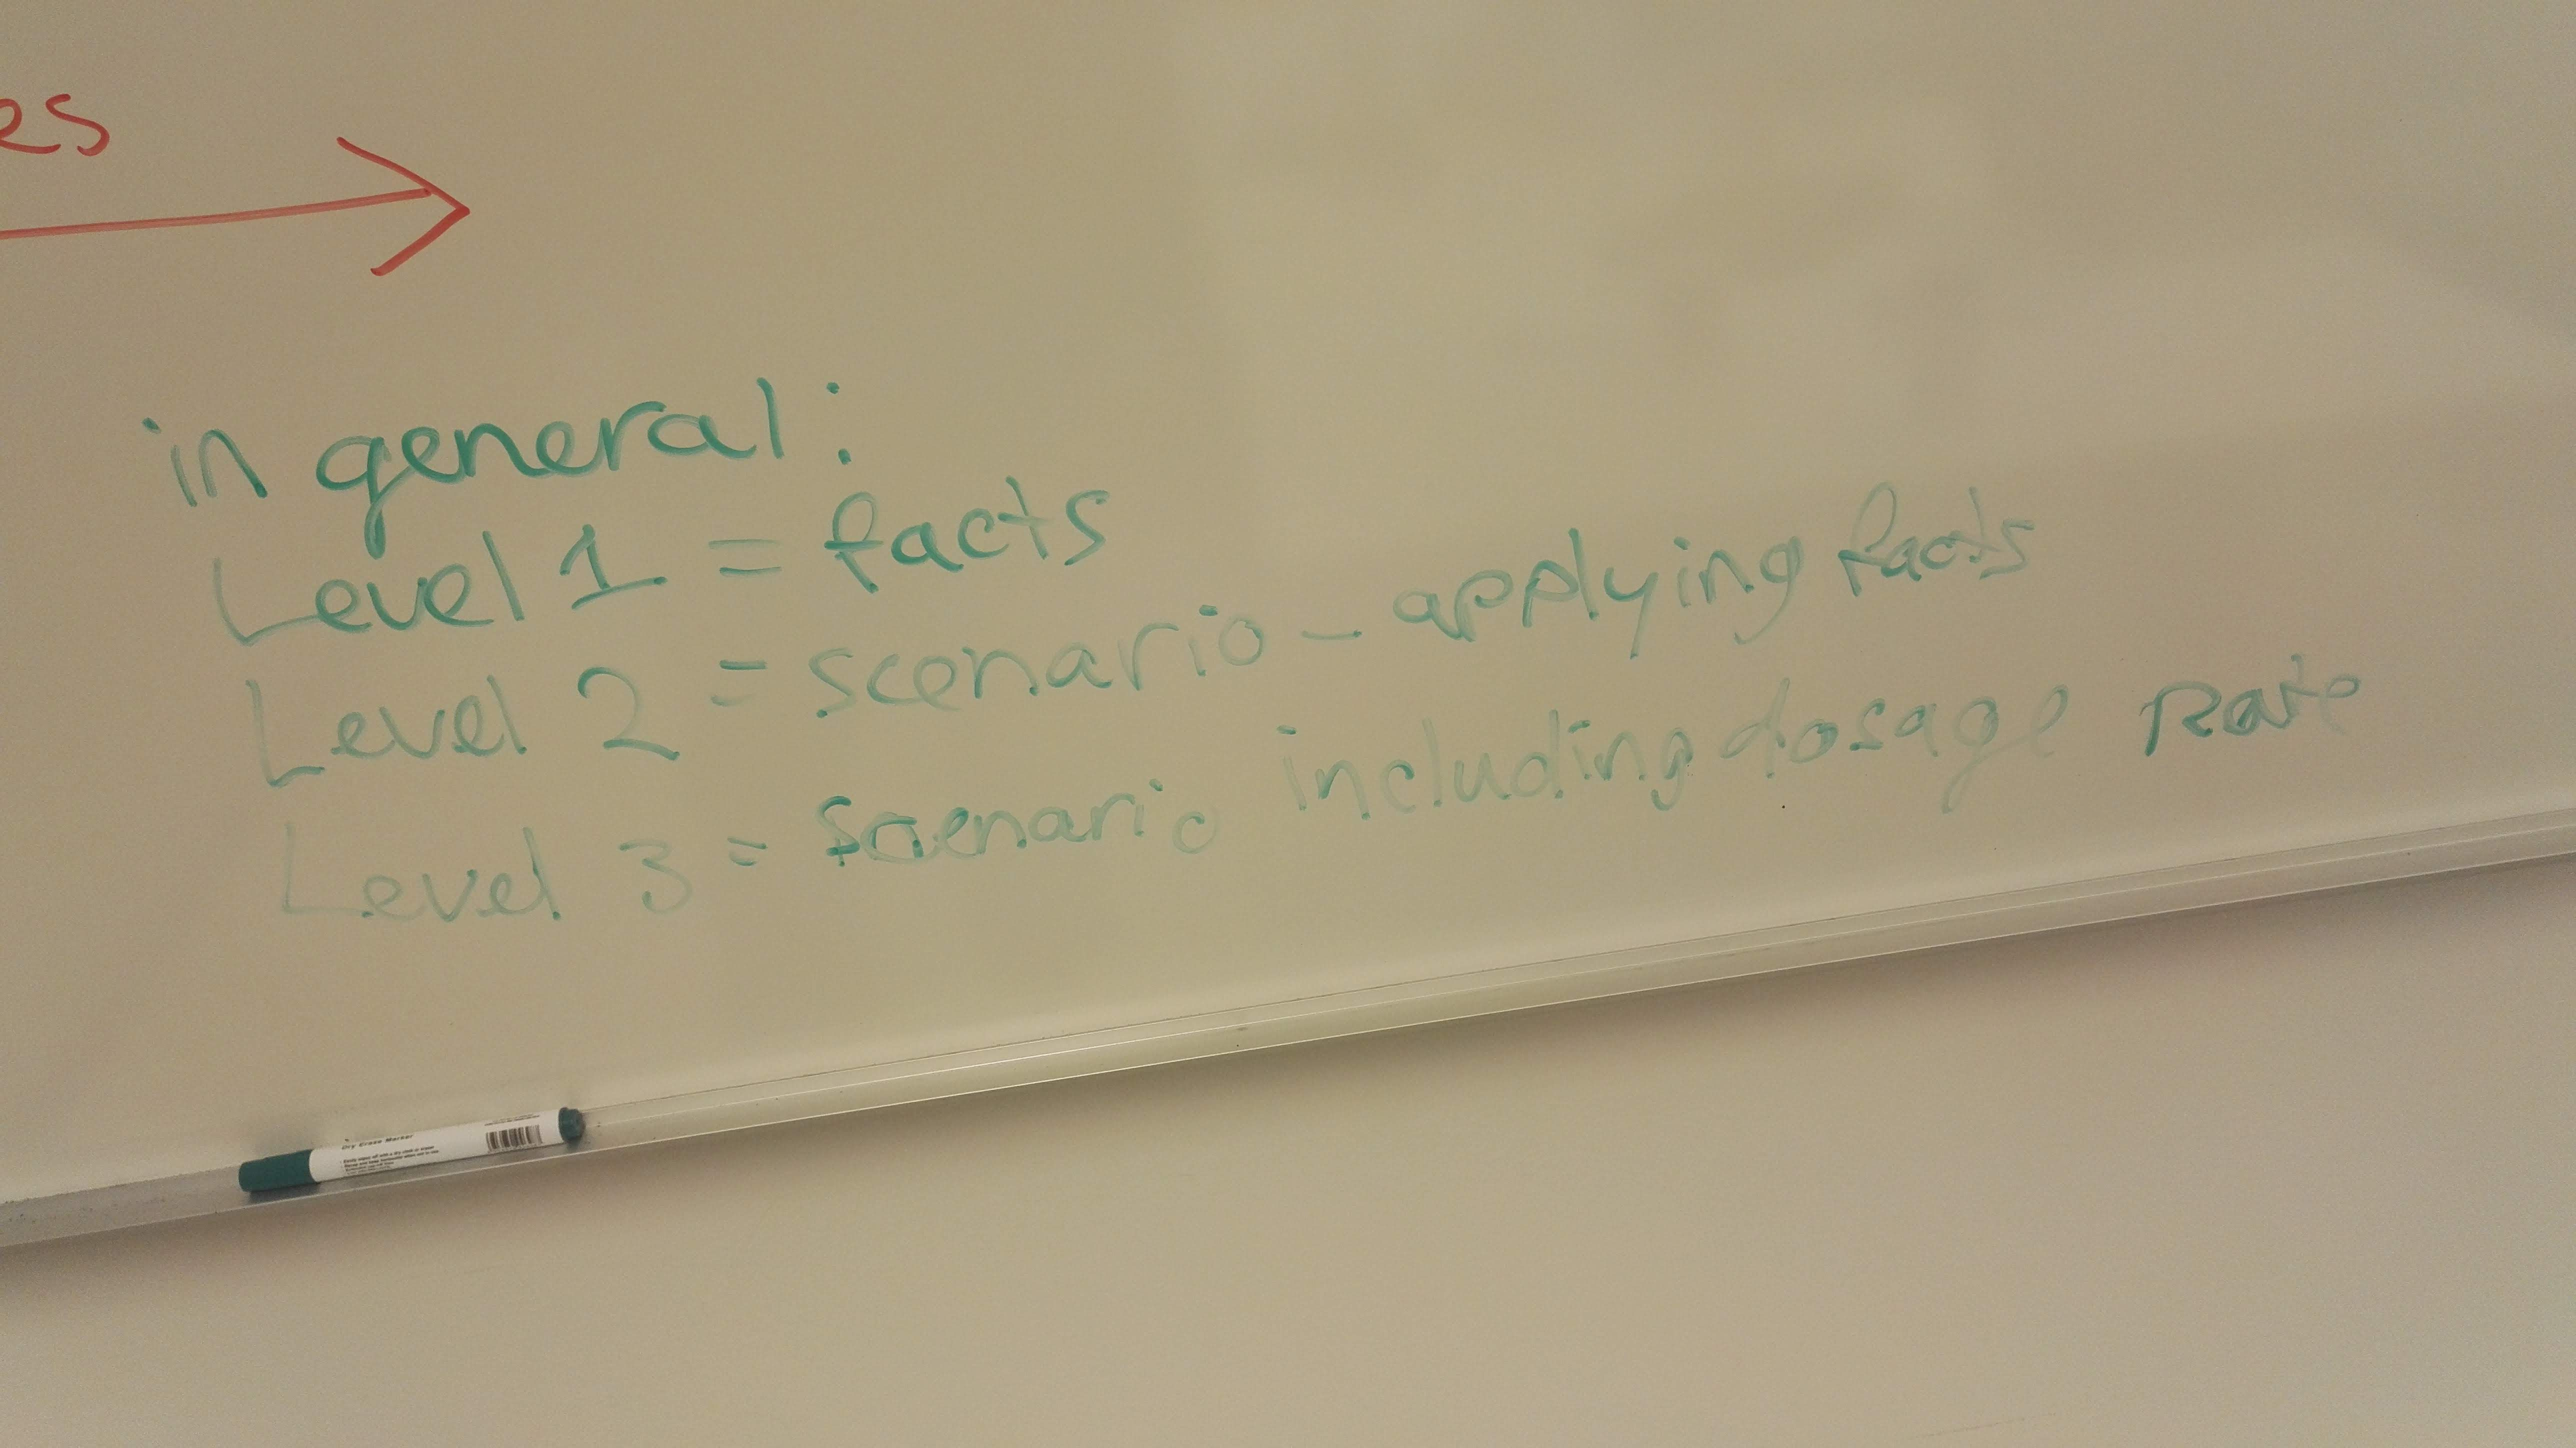
\includegraphics[scale=0.075]{workshop220219-4}
\end{figure}

\begin{figure}[h]
	\caption {Workshop with Yngve Lamo, Rosaline Barendregt, Suresh Kumar Mukhiya, Svein Ivar Lillehaug, Fazle Rabbi and Job Nyangena}
	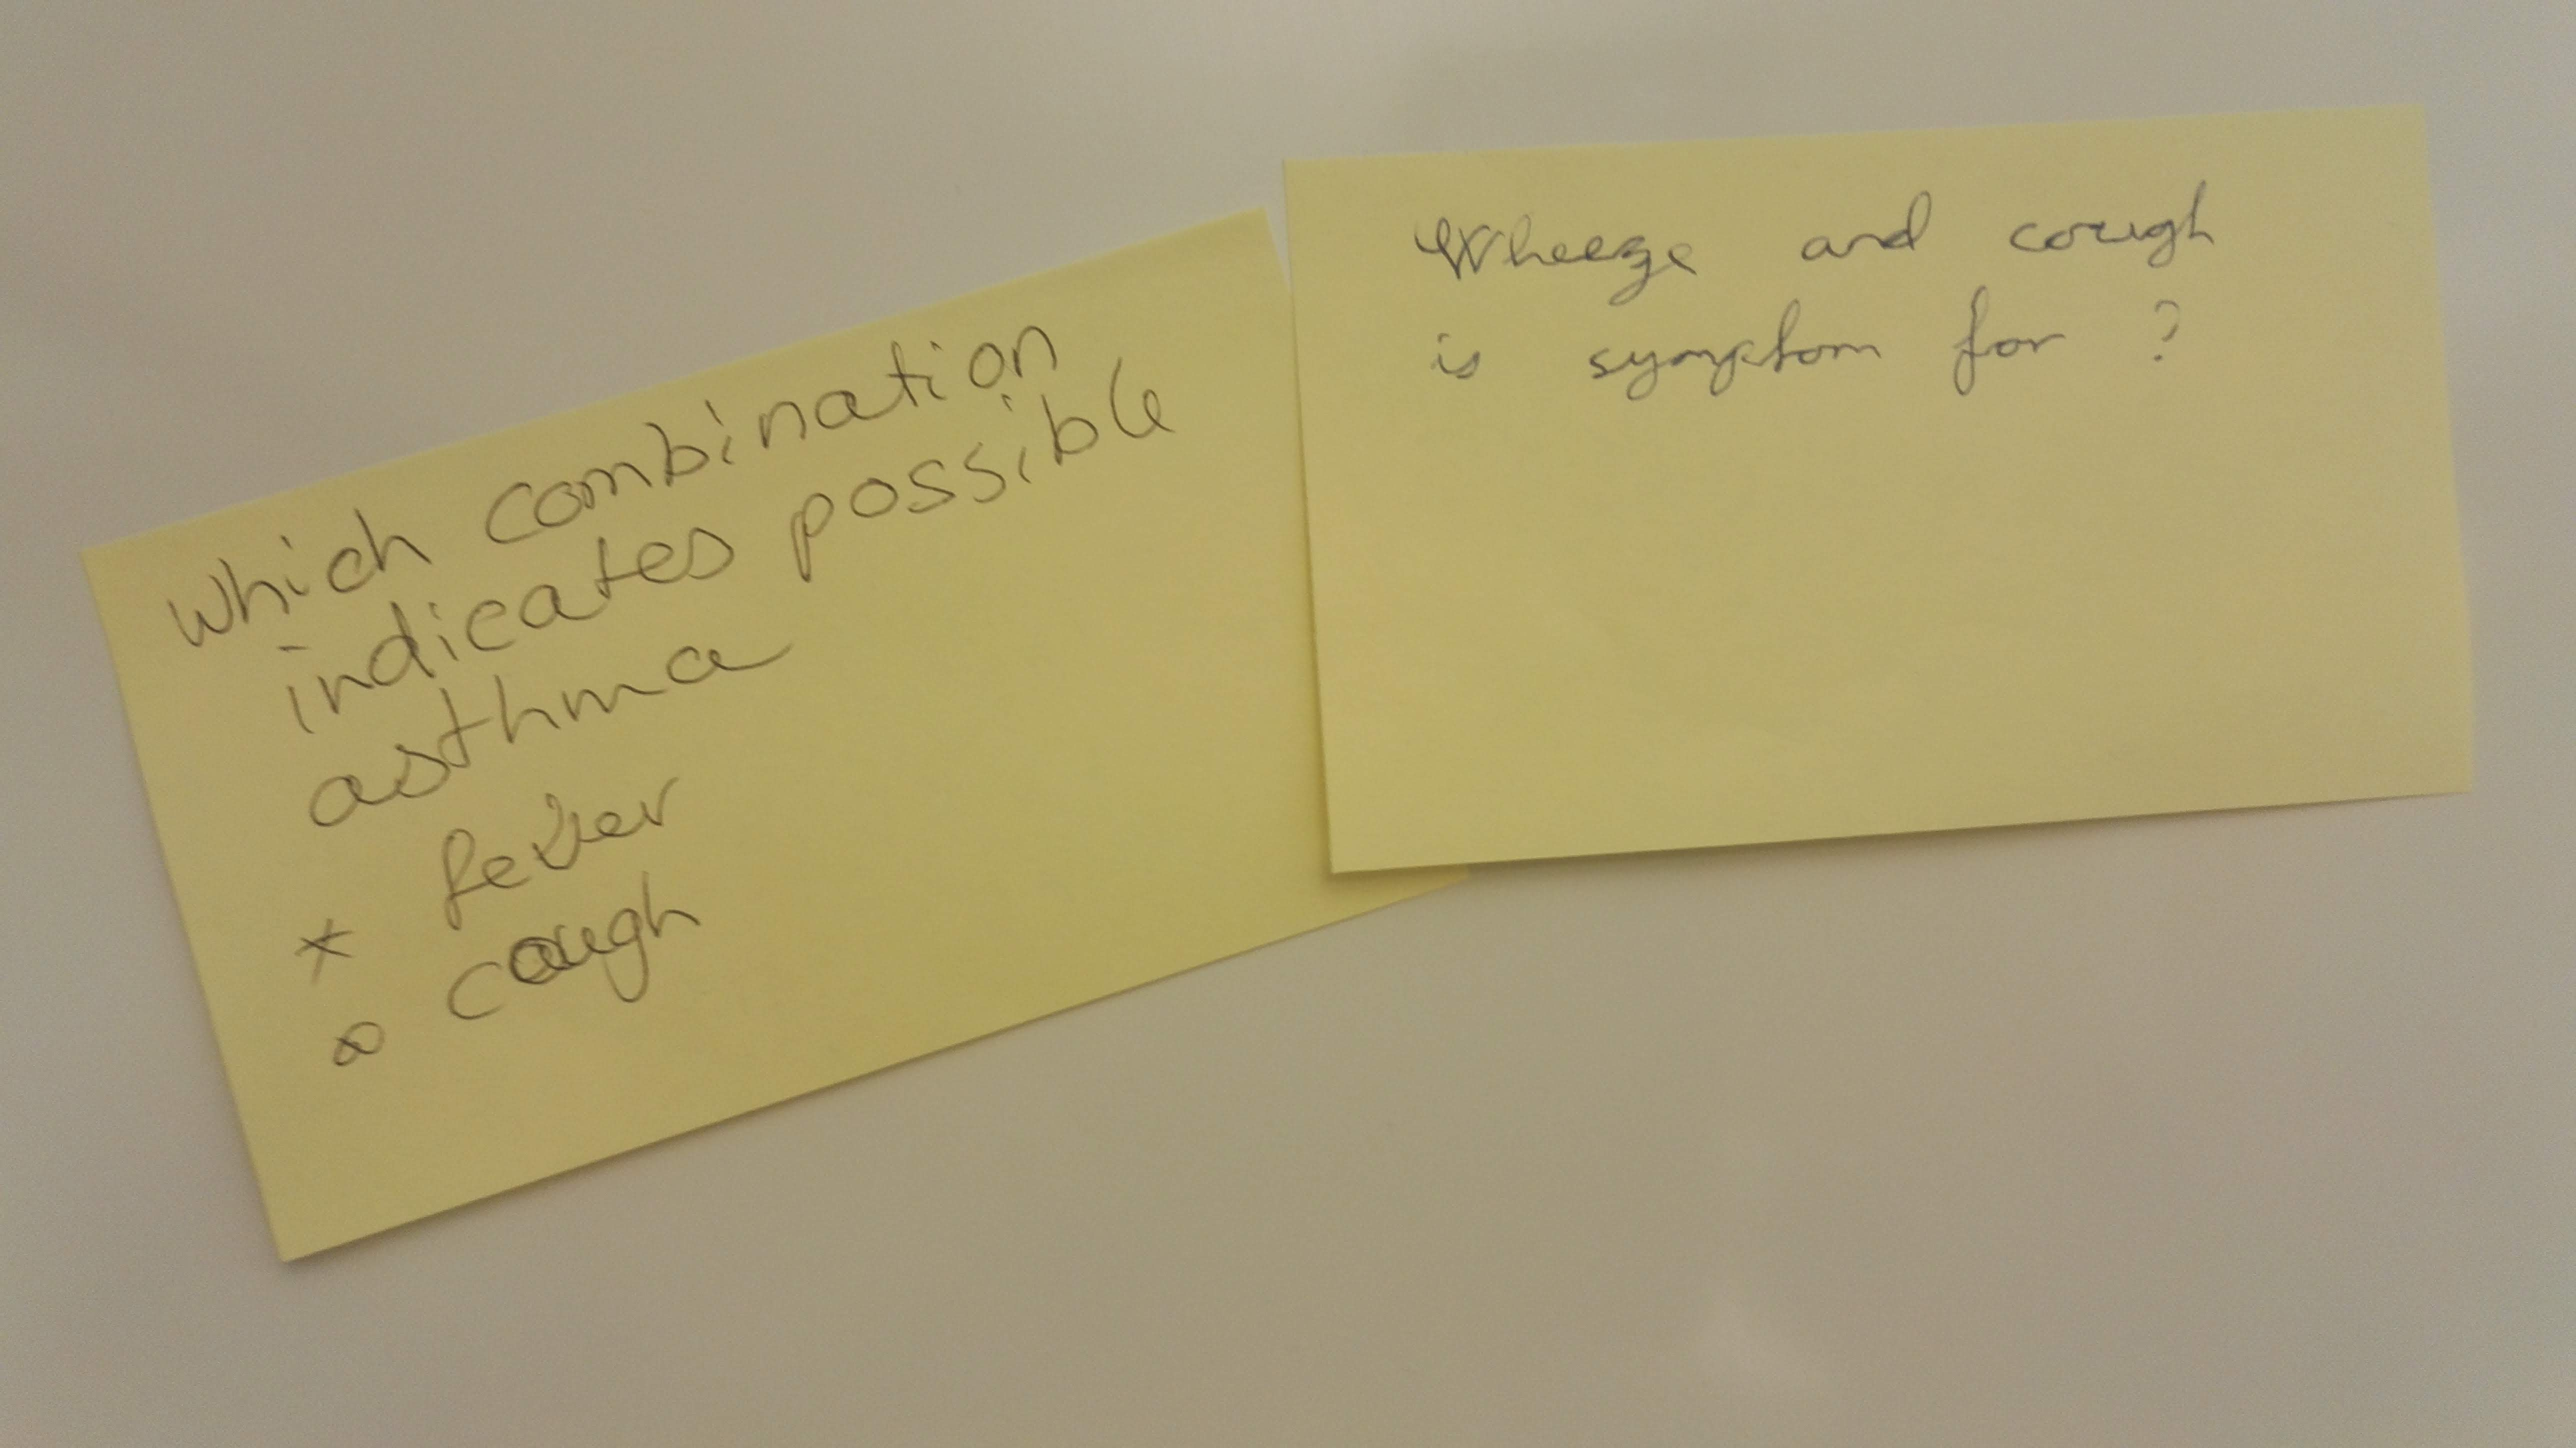
\includegraphics[scale=0.075]{workshop220219-5}
\end{figure}




\chapter{Developing a learning tool for health workers}
\section{Extracting knowledge from the clinical  practice guidelines}
\section{Data models}
\subsection{DPF metamodeling}
\subsection{Entity model}
\subsection{Workflow model}
\subsection{Game model}
\section{Game engine}
\subsection{Reward system}
As each question in a quiz are related to a certain discipline or a certain task, the student will be measured how well he performed on each of these disciplines. For the asthma guideline, we have identified four disciplines. Assessment where the student will be tested in the initial examination. Diagnosis, where the student will determine a diagnosis as well as the severity. Management, where the student will determine which actions should be done to treat and best give the best care to the patient. The last discipline is the follow-up, where the student will be tested in evaluating the treatment, give advise to and educate patient and caregivers, provide the right medication and regular follow-up.

By splitting up the score in disciplines, the student can easily see which areas he is strong and where he needs more training. 



 We can also adapt the questions in each discipline to the students level. If the student has proven to be very good in providing the right amount of medicine to asthma patient, we can provide more difficult questions to challenge the student some more. If he struggles at setting the right diagnose, we can provide more basic questions to strengthen the students basic knowledge. 

\textcolor{red}{The disciplines should be automatically picked from the entity (and worflow?) model.}

\textcolor{red}{The tree structure of discipline scores. Diagnosis have examination, investigation, setting the severity. Management have advises, medication, admit, surgery and so on.}




The student will also be provided with a total score, which will be the average score of each of the disciplines. The student can compare the total score of e.g. the asthma quiz and the jaundice quiz, and see which medical condition he needs to train more on.

Each question will have several answer alternatives the student can choose from. Each answer alternative will have a reward or penalty related to them. The correct answer will have a great reward, while wrong answers will have a small penalty. The quiz author will have the opportunity to specify the rewards, such that he can give even smaller penalties for partly correct answers. The idea of the reward- penalty system is to increase learning. if the student answers wrong the first time, he will be given the possibility to reflect over the question once more or perhaps read the guideline to learn before he commits his second attempt. We are aware that providing a minus score for making an attempt can be very demotivating, but it is to avoid the situation where a student gets the same (or better) score for making ten attempts than only needing one attempt. A small penalty will have a very small impact when the reward per question is high, but in situations where the student performs very poorly and ends with a negative total score, it is possible to adjust this to a small positive score on presentation for the student. Not giving a too harsh feedback for trying to learn.

\textcolor{red}{A solution to having a not very strict game, encouraging to playing and learning, one can also have a very strict examination version. The idea is that after examination, the results will be sent to the lecturer (or a governing body of some kind) to evaluate what the overall knowledge of the students, as well as details of what the students are really good in and where do they struggle. The lecturer can then target the weak of points of the students in one of the next lectures. }


\subsection{Unlocking harder levels at a certain category}
\textcolor{red}{(somewhere in the paper I need to refer to Eides, Kristensens and Lamos paper, and discuss the knowledge, learning and student maps and that they need to prove basic knowledge in some disciplines before they can unlock content in other disciplines.)}
\subsection{Visualization of game statistics}
\subsection{Automatically generating new questions}
\section{The mobile application}
\begin{itemize}
	\item React
	\item React-Native
	\item React-Native-Navigation (Wix)
	\item Redux
	\item React-Redux
	\item Redux-Thunk
	\item Highcharts
	\item Jest
\end{itemize}
\subsection{React-Native and Redux}
\subsection{User interface and flow of the user interaction}
\section{Architecture of the whole system}
\subsection{Visualization}
\section{Evaluation}



\chapter{Discussion}
\section{Research questions}
\section{Limitations of the model}
\begin{itemize}
	\item Can't ask questions like "what are the symptoms for severe asthma?"
	\item Difficult to ask what NOT to do. If the vertex doesn't exist, only an empty string gets returned. Can only be used were we actually have written "don't admit to the hospital" as an example with hospitalization.
	\item The inheritance makes it difficult to generalize some questions. We can't make a template which asks about the Rate a medicine should be taken with. We need to specifically ask for that medicine. To be able to ask for a general medicine, one solution can be to introduce a new tag which compares the substring of the type of the vertex. Another solution is to use the meta model and not the instance model. We don't use inheritance on diagnosis because of this.
	\item To avoid the problem described in the previous point, we don't use inheritance on Diagnosis. A limitation here is that  
	a patient can only have one diagnosis.
\end{itemize}
\section{Observations}
\section{Challenges}
\section{Reflection}



\chapter{Conclusions}
\section{Further research and development}


\backmatter
% bibliography, glossary and index would go here.
\end{document}